\documentclass[12pt]{beamer}

% Theme & Colors
\usetheme{Madrid} % Try: Berlin, Copenhagen, CambridgeUS, Warsaw...
\usecolortheme{dolphin} % Try: seahorse, crane, beaver...

% Encoding & Fonts
\usepackage[utf8]{inputenc}
\usepackage[T1]{fontenc}
\usepackage{lmodern} % Better font
\usepackage{luatexja}
\usepackage{luatexja-fontspec}
\usepackage{amsmath,amssymb,mathtools,ascmac,amsthm,amscd,tikz-cd}
\usetikzlibrary{arrows.meta,calc,quotes,angles}
\setmainjfont{Noto Sans CJK JP}
% Title Information
\newcommand{\circnum}[2][]{%
  \tikz[baseline=(n.base)] \node (n) [circnum,#1]{#2};%
}
\title[五心]{三角形の五心}
\date{\today}

\begin{document}
% Title Page
\begin{frame}
  \titlepage
\end{frame}

% Outline
\begin{frame}{三角形の五心}
  \tableofcontents
\end{frame}

% Section 1
\section{重心}
\begin{frame}{対辺}
  \begin{block}{対辺の定義}
		頂点に向かい合う辺を対辺という.
  \end{block}
	\begin{center}
	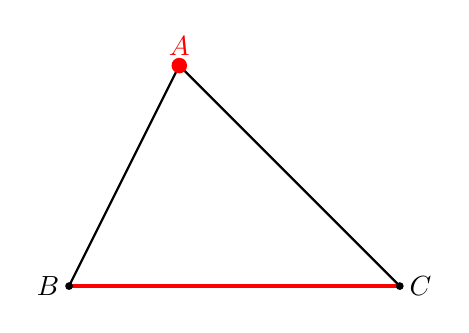
\begin{tikzpicture}[scale=1.4]
  % Define the vertices
  \coordinate (B) at (0,0);
  \coordinate (C) at (3,0);
  \coordinate (A) at (1,2);
  % Draw the triangle
  \draw[thick] (A)--(B);
  \draw[thick] (A)--(C);
  \draw[red,very thick] (B)--(C);
  % Mark the points
	\fill[red] (A) circle (2pt) node[above] {$A$};
  \fill (B) circle (1pt) node[left] {$B$};
  \fill (C) circle (1pt) node[right] {$C$};
\end{tikzpicture}
\end{center}
例.頂点$A$の対辺は辺$BC$
\end{frame}

\begin{frame}{中線}
  \begin{block}{中線の定義}
		頂点とその対辺の中点を結ぶ線分を中線という.
  \end{block}
	\begin{center}
	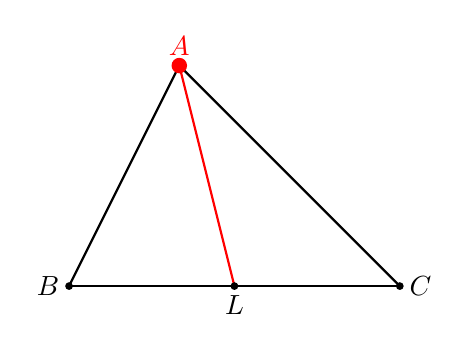
\begin{tikzpicture}[scale=1.4]
  % Define the vertices
  \coordinate (B) at (0,0);
  \coordinate (C) at (3,0);
  \coordinate (A) at (1,2);
  \coordinate (L) at (1.5,0);
  % Draw the triangle
  \draw[thick] (A)--(B);
  \draw[thick] (A)--(C);
  \draw[thick] (B)--(C);
  \draw[thick,red] (A)--(L);
  % Mark the points
	\fill[red] (A) circle (2pt) node[above] {$A$};
  \fill (B) circle (1pt) node[left] {$B$};
  \fill (C) circle (1pt) node[right] {$C$};
  \fill (L) circle (1pt) node[below] {$L$};
\end{tikzpicture}
\[BL = LC\]
\end{center}
\end{frame}

\begin{frame}{重心}
  \begin{block}{重心の定義}
		三角形の3本の中線は1点で交わり,その点を重心と呼ぶ.\\
  \end{block}
	\begin{center}
	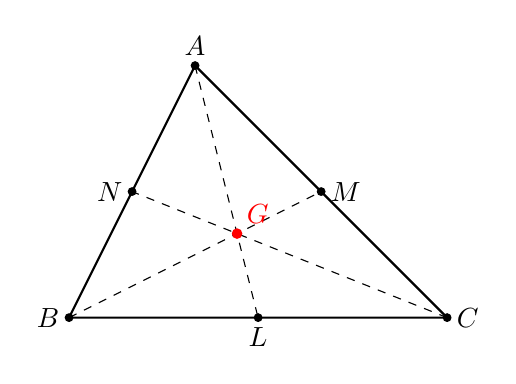
\begin{tikzpicture}[scale=1.6]
  % Define the vertices
  \coordinate (B) at (0,0);
  \coordinate (C) at (3,0);
  \coordinate (A) at (1,2);
  \coordinate (L) at ($(B)!0.5!(C)$);
  \coordinate (M) at ($(A)!0.5!(C)$);
  \coordinate (N) at ($(A)!0.5!(B)$);
  % Draw the triangle
  \draw[thick] (A)--(B)--(C)--cycle;

  % Compute centroid G = (A+B+C)/3
  \coordinate (G) at (4/3,2/3);

  % Draw medians
  \draw[dashed] (A)--($(B)!0.5!(C)$);
  \draw[dashed] (B)--($(A)!0.5!(C)$);
  \draw[dashed] (C)--($(A)!0.5!(B)$);
  % Mark the points
  \fill (A) circle (1pt) node[above] {$A$};
  \fill (B) circle (1pt) node[left] {$B$};
  \fill (C) circle (1pt) node[right] {$C$};
  \fill (L) circle (1pt) node[below] {$L$};
  \fill (M) circle (1pt) node[right] {$M$};
  \fill (N) circle (1pt) node[left] {$N$};
  \fill[red] (G) circle (1.2pt) node[above right] {$G$};
\end{tikzpicture}
\end{center}
$\longrightarrow $ 3つの中線が1点で交わるということは,明らかではない.
\end{frame}

\begin{frame}{重心の存在}
	\begin{block}{定理3}
		三角形の3本の中線は1点で交わる.\\
		さらに,その交点(重心)は各中線を$2:1$に内分する.
  \end{block}
	\begin{center}
	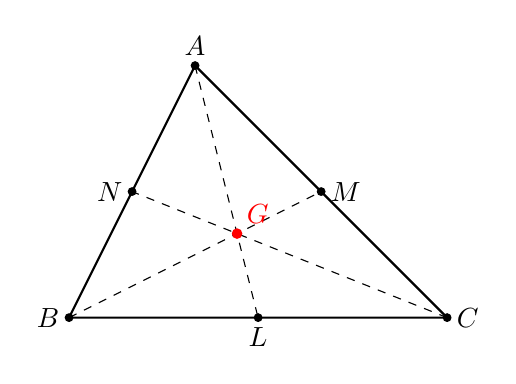
\begin{tikzpicture}[scale=1.6]
  % Define the vertices
  \coordinate (B) at (0,0);
  \coordinate (C) at (3,0);
  \coordinate (A) at (1,2);
  \coordinate (L) at ($(B)!0.5!(C)$);
  \coordinate (M) at ($(A)!0.5!(C)$);
  \coordinate (N) at ($(A)!0.5!(B)$);
  % Draw the triangle
  \draw[thick] (A)--(B)--(C)--cycle;

  % Compute centroid G = (A+B+C)/3
  \coordinate (G) at (4/3,2/3);

  % Draw medians
  \draw[dashed] (A)--($(B)!0.5!(C)$);
  \draw[dashed] (B)--($(A)!0.5!(C)$);
  \draw[dashed] (C)--($(A)!0.5!(B)$);
  % Mark the points
  \fill (A) circle (1pt) node[above] {$A$};
  \fill (B) circle (1pt) node[left] {$B$};
  \fill (C) circle (1pt) node[right] {$C$};
  \fill (L) circle (1pt) node[below] {$L$};
  \fill (M) circle (1pt) node[right] {$M$};
  \fill (N) circle (1pt) node[left] {$N$};
  \fill[red] (G) circle (1.2pt) node[above right] {$G$};
\end{tikzpicture}
\end{center}
\end{frame}

\begin{frame}{証明}
	$NC$と$BM$の交点を$G$とする.
	\begin{center}
	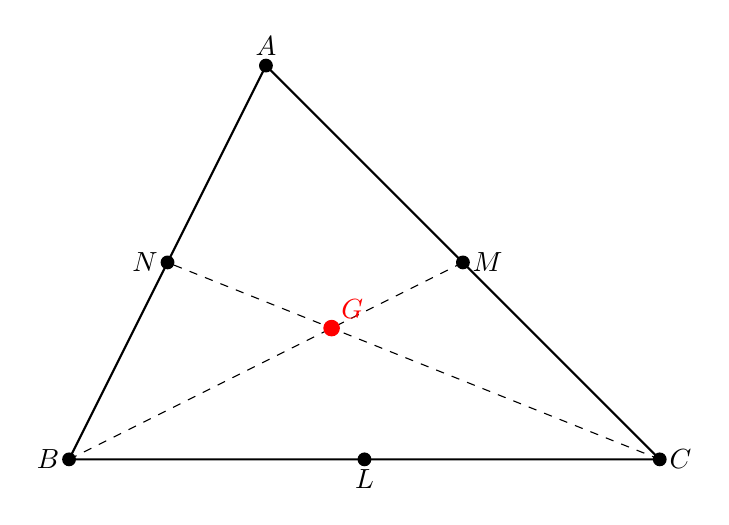
\begin{tikzpicture}[scale=2.5]
  % Define the vertices
  \coordinate (B) at (0,0);
  \coordinate (C) at (3,0);
  \coordinate (A) at (1,2);
  \coordinate (L) at ($(B)!0.5!(C)$);
  \coordinate (M) at ($(A)!0.5!(C)$);
  \coordinate (N) at ($(A)!0.5!(B)$);
  % Draw the triangle
  \draw[thick] (A)--(B)--(C)--cycle;

  % Compute centroid G = (A+B+C)/3
  \coordinate (G) at (4/3,2/3);

  % Draw medians
 % \draw[dashed] (A)--($(B)!0.5!(C)$);
  \draw[dashed] (B)--($(A)!0.5!(C)$);
  \draw[dashed] (C)--($(A)!0.5!(B)$);
  % Mark the points
  \fill (A) circle (1pt) node[above] {$A$};
  \fill (B) circle (1pt) node[left] {$B$};
  \fill (C) circle (1pt) node[right] {$C$};
  \fill (L) circle (1pt) node[below] {$L$};
  \fill (M) circle (1pt) node[right] {$M$};
  \fill (N) circle (1pt) node[left] {$N$};
  \fill[red] (G) circle (1.2pt) node[above right] {$G$};
\end{tikzpicture}
\end{center}
\end{frame}

\begin{frame}{証明}
	\begin{center}
	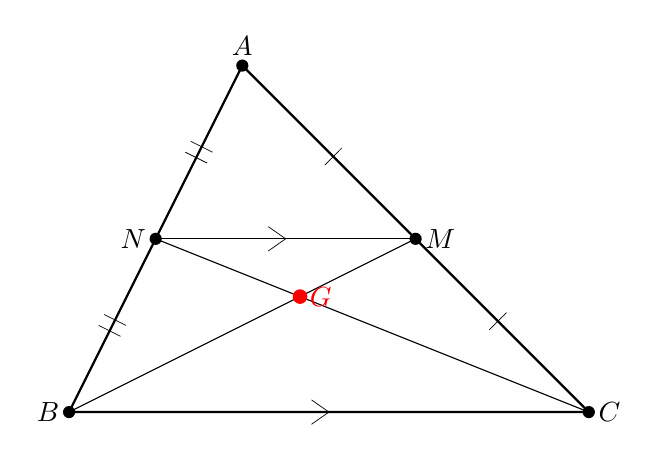
\begin{tikzpicture}[scale=2.2]
  % Define the vertices
  \coordinate (B) at (0,0);
  \coordinate (C) at (3,0);
  \coordinate (A) at (1,2);
  \coordinate (L) at ($(B)!0.5!(C)$);
  \coordinate (M) at ($(A)!0.5!(C)$);
  \coordinate (N) at ($(A)!0.5!(B)$);
  % Draw the triangle
  \draw[thick] (A)--(B)--(C)--cycle;

	\draw [line width=0.25pt] ($(N)!0.5!(A)!1pt!(N)!2pt!90:(N)$) -- ($(N)!0.5!(A)!1pt!(N)!2pt!90:(A)$) ($(N)!0.5!(A)!1pt!(A)!2pt!90:(N)$) -- ($(N)!0.5!(A)!1pt!(A)!2pt!90:(A)$);
	\draw [line width=0.25pt] ($(N)!0.5!(B)!1pt!(N)!2pt!90:(N)$) -- ($(N)!0.5!(B)!1pt!(N)!2pt!90:(B)$) ($(N)!0.5!(B)!1pt!(B)!2pt!90:(N)$) -- ($(N)!0.5!(B)!1pt!(B)!2pt!90:(B)$);
	\draw [line width=0.25pt] ($(M)!0.5!(A)!1pt!(M)!2pt!90:(M)$) -- ($(M)!0.5!(A)!1pt!(M)!2pt!90:(A)$) ;
	\draw [line width=0.25pt] ($(M)!0.5!(C)!1pt!(M)!2pt!90:(M)$) -- ($(M)!0.5!(C)!1pt!(M)!2pt!90:(C)$) ;

	\draw [line width=0.25pt] ($(N)!0.5!(M)!3.5pt!145:(M)$) -- ($(N)!0.5!(M)$) -- ($(N)!0.5!(M)!3.5pt!-145:(M)$);
	\draw [line width=0.25pt] ($(B)!0.5!(C)!3.5pt!145:(C)$) -- ($(B)!0.5!(C)$) -- ($(B)!0.5!(C)!3.5pt!-145:(C)$);
  % Compute centroid G = (A+B+C)/3
  \coordinate (G) at (4/3,2/3);

  % Draw medians
 % \draw[dashed] (A)--($(B)!0.5!(C)$);
  \draw[] (B)--($(A)!0.5!(C)$);
  \draw[] (C)--($(A)!0.5!(B)$);
  \draw[] (N)--(M);
  % Mark the points
  \fill (A) circle (1pt) node[above] {$A$};
  \fill (B) circle (1pt) node[left] {$B$};
  \fill (C) circle (1pt) node[right] {$C$};
  %\fill (L) circle (1pt) node[below] {$L$};
  \fill (M) circle (1pt) node[right] {$M$};
  \fill (N) circle (1pt) node[left] {$N$};
  \fill[red] (G) circle (1.2pt) node[right] {$G$};
\end{tikzpicture}\\
平行線と線分の比の性質より,\\
$AB:AN = AC : AM = 2 : 1$なので,$NM// BC$
\end{center}
\end{frame}

\begin{frame}{証明}
	\begin{center}
	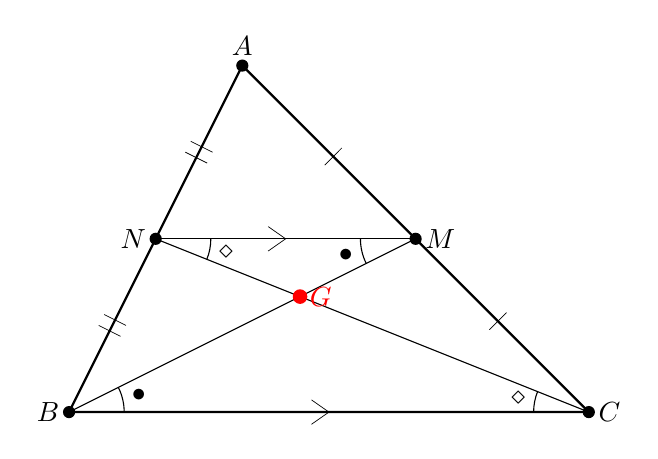
\begin{tikzpicture}[scale=2.2]
  % Define the vertices
  \coordinate (B) at (0,0);
  \coordinate (C) at (3,0);
  \coordinate (A) at (1,2);
  \coordinate (L) at ($(B)!0.5!(C)$);
  \coordinate (M) at ($(A)!0.5!(C)$);
  \coordinate (N) at ($(A)!0.5!(B)$);
  % Draw the triangle
  \draw[thick] (A)--(B)--(C)--cycle;

	\draw [line width=0.25pt] ($(N)!0.5!(A)!1pt!(N)!2pt!90:(N)$) -- ($(N)!0.5!(A)!1pt!(N)!2pt!90:(A)$) ($(N)!0.5!(A)!1pt!(A)!2pt!90:(N)$) -- ($(N)!0.5!(A)!1pt!(A)!2pt!90:(A)$);
	\draw [line width=0.25pt] ($(N)!0.5!(B)!1pt!(N)!2pt!90:(N)$) -- ($(N)!0.5!(B)!1pt!(N)!2pt!90:(B)$) ($(N)!0.5!(B)!1pt!(B)!2pt!90:(N)$) -- ($(N)!0.5!(B)!1pt!(B)!2pt!90:(B)$);
	\draw [line width=0.25pt] ($(M)!0.5!(A)!1pt!(M)!2pt!90:(M)$) -- ($(M)!0.5!(A)!1pt!(M)!2pt!90:(A)$) ;
	\draw [line width=0.25pt] ($(M)!0.5!(C)!1pt!(M)!2pt!90:(M)$) -- ($(M)!0.5!(C)!1pt!(M)!2pt!90:(C)$) ;

	\draw [line width=0.25pt] ($(N)!0.5!(M)!3.5pt!145:(M)$) -- ($(N)!0.5!(M)$) -- ($(N)!0.5!(M)!3.5pt!-145:(M)$);
	\draw [line width=0.25pt] ($(B)!0.5!(C)!3.5pt!145:(C)$) -- ($(B)!0.5!(C)$) -- ($(B)!0.5!(C)!3.5pt!-145:(C)$);
  % Compute centroid G = (A+B+C)/3
  \coordinate (G) at (4/3,2/3);

  % Draw medians
 % \draw[dashed] (A)--($(B)!0.5!(C)$);
  \draw[] (B)--($(A)!0.5!(C)$);
  \draw[] (C)--($(A)!0.5!(B)$);
  \draw[] (N)--(M);
  % Mark the points
  \fill (A) circle (1pt) node[above] {$A$};
  \fill (B) circle (1pt) node[left] {$B$};
  \fill (C) circle (1pt) node[right] {$C$};
  %\fill (L) circle (1pt) node[below] {$L$};
  \fill (M) circle (1pt) node[right] {$M$};
  \fill (N) circle (1pt) node[left] {$N$};
  \fill[red] (G) circle (1.2pt) node[right] {$G$};
	 \path pic["$\bullet$",draw,angle radius=7mm,angle eccentricity=1.3] {angle = C--B--G};
	 \path pic["$\bullet$",draw,angle radius=7mm,angle eccentricity=1.3] {angle = N--M--G};
	 \path pic["$\diamond$",draw,angle radius=7mm,angle eccentricity=1.3] {angle = G--N--M};
	 \path pic["$\diamond$",draw,angle radius=7mm,angle eccentricity=1.3] {angle = G--C--B};
\end{tikzpicture}\\
平行線の錯角が等しいことから,\triangle BGC $\backsim$ \triangle MGN \\
BC : NM = 2 : 1だから,BG : GM = 2 : 1.
\end{center}
\end{frame}

\begin{frame}{証明}
	$AL$と$BM$の交点を$H$とする.
	\begin{center}
	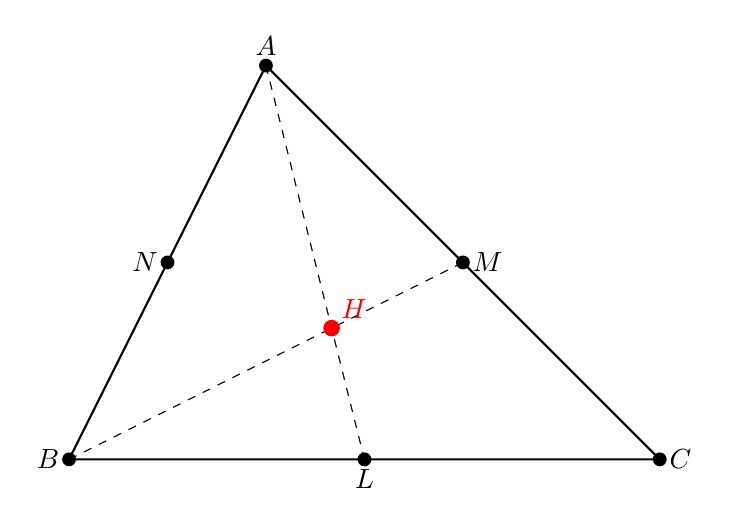
\begin{tikzpicture}[scale=2.5]
  % Define the vertices
  \coordinate (B) at (0,0);
  \coordinate (C) at (3,0);
  \coordinate (A) at (1,2);
  \coordinate (L) at ($(B)!0.5!(C)$);
  \coordinate (M) at ($(A)!0.5!(C)$);
  \coordinate (N) at ($(A)!0.5!(B)$);
  % Draw the triangle
  \draw[thick] (A)--(B)--(C)--cycle;

  % Compute centroid G = (A+B+C)/3
  \coordinate (G) at (4/3,2/3);

  % Draw medians
	 \draw[dashed] (A)--($(B)!0.5!(C)$);
  \draw[dashed] (B)--($(A)!0.5!(C)$);
  %\draw[dashed] (C)--($(A)!0.5!(B)$);
  % Mark the points
  \fill (A) circle (1pt) node[above] {$A$};
  \fill (B) circle (1pt) node[left] {$B$};
  \fill (C) circle (1pt) node[right] {$C$};
  \fill (L) circle (1pt) node[below] {$L$};
  \fill (M) circle (1pt) node[right] {$M$};
  \fill (N) circle (1pt) node[left] {$N$};
  \fill[red] (G) circle (1.2pt) node[above right] {$H$};
\end{tikzpicture}
\end{center}
\end{frame}

\begin{frame}{証明}
	$G$の場合と同様にして,
	\begin{center}
	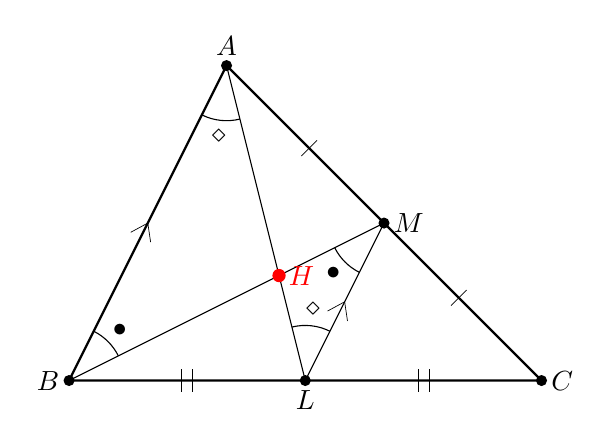
\begin{tikzpicture}[scale=2.0]
  % Define the vertices
  \coordinate (B) at (0,0);
  \coordinate (C) at (3,0);
  \coordinate (A) at (1,2);
  \coordinate (L) at ($(B)!0.5!(C)$);
  \coordinate (M) at ($(A)!0.5!(C)$);
  \coordinate (N) at ($(A)!0.5!(B)$);
  % Draw the triangle
  \draw[thick] (A)--(B)--(C)--cycle;

	\draw [line width=0.25pt] ($(L)!0.5!(C)!1pt!(L)!2pt!90:(L)$) -- ($(L)!0.5!(C)!1pt!(L)!2pt!90:(C)$) ($(L)!0.5!(C)!1pt!(C)!2pt!90:(L)$) -- ($(L)!0.5!(C)!1pt!(C)!2pt!90:(C)$);
	\draw [line width=0.25pt] ($(L)!0.5!(B)!1pt!(L)!2pt!90:(L)$) -- ($(L)!0.5!(B)!1pt!(L)!2pt!90:(B)$) ($(L)!0.5!(B)!1pt!(B)!2pt!90:(L)$) -- ($(L)!0.5!(B)!1pt!(B)!2pt!90:(B)$);
	\draw [line width=0.25pt] ($(M)!0.5!(A)!1pt!(M)!2pt!90:(M)$) -- ($(M)!0.5!(A)!1pt!(M)!2pt!90:(A)$) ;
	\draw [line width=0.25pt] ($(M)!0.5!(C)!1pt!(M)!2pt!90:(M)$) -- ($(M)!0.5!(C)!1pt!(M)!2pt!90:(C)$) ;

	\draw [line width=0.25pt] ($(L)!0.5!(M)!3.5pt!145:(M)$) -- ($(L)!0.5!(M)$) -- ($(L)!0.5!(M)!3.5pt!-145:(M)$);
	\draw [line width=0.25pt] ($(B)!0.5!(A)!3.5pt!145:(A)$) -- ($(B)!0.5!(A)$) -- ($(B)!0.5!(A)!3.5pt!-145:(A)$);
  % Compute centroid G = (A+B+C)/3
  \coordinate (G) at (4/3,2/3);

  % Draw medians
 % \draw[dashed] (A)--($(B)!0.5!(C)$);
  \draw[] (B)--(M);
  \draw[] (A)--(L);
  \draw[] (M)--(L);
  % Mark the points
  \fill (A) circle (1pt) node[above] {$A$};
  \fill (B) circle (1pt) node[left] {$B$};
  \fill (C) circle (1pt) node[right] {$C$};
  \fill (L) circle (1pt) node[below] {$L$};
  \fill (M) circle (1pt) node[right] {$M$};
  %\fill (N) circle (1pt) node[left] {$N$};
  \fill[red] (G) circle (1.2pt) node[right] {$H$};
	 \path pic["$\bullet$",draw,angle radius=7mm,angle eccentricity=1.3] {angle = G--B--A};
	 \path pic["$\bullet$",draw,angle radius=7mm,angle eccentricity=1.3] {angle = G--M--L};
	 \path pic["$\diamond$",draw,angle radius=7mm,angle eccentricity=1.3] {angle = B--A--L};
	 \path pic["$\diamond$",draw,angle radius=7mm,angle eccentricity=1.3] {angle = M--L--A};
\end{tikzpicture}\\
AB : ML = 2 : 1だから,BH : HM = 2 : 1.がわかる.\\
GもHもBMを2 : 1 に内分する点なのでG = H.\blacksquare\\
(あとで証明するチェバの定理の逆を使えば明らか.)
\end{center}
\end{frame}
% Section 2
\section{外心}
\begin{frame}{外心の定義}
  \begin{block}{外心の定義}
		三角形の垂直二等分線は1点で交わり,外心と呼ぶ.
  \end{block}
	\begin{center}
	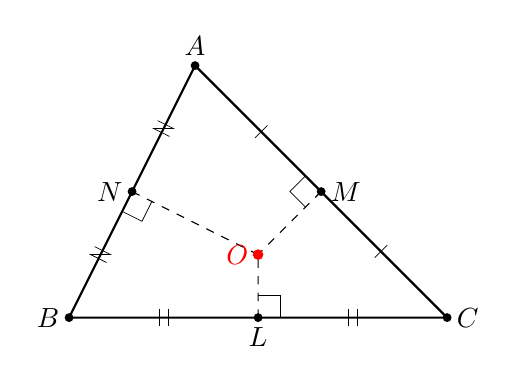
\begin{tikzpicture}[scale=1.6]
  % Define the vertices
  \coordinate (B) at (0,0);
  \coordinate (C) at (3,0);
  \coordinate (A) at (1,2);
  \coordinate (L) at ($(B)!0.5!(C)$);
  \coordinate (M) at ($(A)!0.5!(C)$);
  \coordinate (N) at ($(A)!0.5!(B)$);

  % Draw the triangle
  \draw[thick] (A)--(B)--(C)--cycle;

  % Compute centroid G = (A+B+C)/3
  \coordinate (O) at (3/2,1/2);
	\draw [line width=0.25pt] ($(L)!5pt!(C)$) -- ($(L)!5pt!(C)!5pt!90:(C)$) -- ($(L)!5pt!90:(C)$);
	\draw [line width=0.25pt] ($(M)!5pt!(A)$) -- ($(M)!5pt!(A)!5pt!90:(A)$) -- ($(M)!5pt!90:(A)$);
	\draw [line width=0.25pt] ($(N)!5pt!(B)$) -- ($(N)!5pt!(B)!5pt!90:(B)$) -- ($(N)!5pt!90:(B)$);

	\draw [line width=0.25pt] ($(L)!0.5!(C)!1pt!(L)!2pt!90:(L)$) -- ($(L)!0.5!(C)!1pt!(L)!2pt!90:(C)$) ($(L)!0.5!(C)!1pt!(C)!2pt!90:(L)$) -- ($(L)!0.5!(C)!1pt!(C)!2pt!90:(C)$);
	\draw [line width=0.25pt] ($(L)!0.5!(B)!1pt!(L)!2pt!90:(L)$) -- ($(L)!0.5!(B)!1pt!(L)!2pt!90:(B)$) ($(L)!0.5!(B)!1pt!(B)!2pt!90:(L)$) -- ($(L)!0.5!(B)!1pt!(B)!2pt!90:(B)$);
	\draw [line width=0.25pt] ($(M)!0.5!(A)!1pt!(M)!2pt!90:(M)$) -- ($(M)!0.5!(A)!1pt!(M)!2pt!90:(A)$) ;
	\draw [line width=0.25pt] ($(M)!0.5!(C)!1pt!(M)!2pt!90:(M)$) -- ($(M)!0.5!(C)!1pt!(M)!2pt!90:(C)$) ;
	\draw [line width=0.25pt] ($(N)!0.5!(A)!1pt!(N)!2pt!90:(N)$) -- ($(N)!0.5!(A)!1pt!(N)!2pt!90:(A)$) -- ($(N)!0.5!(A)!1pt!(A)!2pt!90:(N)$) -- ($(N)!0.5!(A)!1pt!(A)!2pt!90:(A)$);
	\draw [line width=0.25pt] ($(N)!0.5!(B)!1pt!(N)!2pt!90:(N)$) -- ($(N)!0.5!(B)!1pt!(N)!2pt!90:(B)$) -- ($(N)!0.5!(B)!1pt!(B)!2pt!90:(N)$) -- ($(N)!0.5!(B)!1pt!(B)!2pt!90:(B)$);

	 %\draw (O) circle (1.58);
  % Draw medians
  \draw[dashed] (L)--(O);
  \draw[dashed] (M)--(O);
  \draw[dashed] (N)--(O);
  %\draw[dashed] (A)--(O);

  % Mark the points
  \fill (A) circle (1pt) node[above] {$A$};
  \fill (B) circle (1pt) node[left] {$B$};
  \fill (C) circle (1pt) node[right] {$C$};
  \fill (L) circle (1pt) node[below] {$L$};
  \fill (M) circle (1pt) node[right] {$M$};
  \fill (N) circle (1pt) node[left] {$N$};
  \fill[red] (O) circle (1.2pt) node[left] {$O$};
\end{tikzpicture}
\end{center}
\end{frame}

\begin{frame}{証明}
	\begin{block}{定理4}
		三角形の3辺の垂直二等分線は1点で交わる.
	\end{block}
	\begin{block}{準備}
		$P$が線分$AB$の垂直二等分線上にある$\Longleftrightarrow$ $PA = PB$
	\end{block}
	\begin{center}
		\begin{tikzpicture}[scale = 1.6]
  \coordinate (A) at (0,0);
  \coordinate (B) at (3,0);
  \coordinate (P) at (1.5,1.5);
  \coordinate (H) at (1.5,0);
  \draw[] (A)--(B);
  \draw[] (P)--(H);
  \draw[dashed] (A)--(P);
  \draw[dashed] (B)--(P);
  \fill (P) circle (1pt) node[above] {$P$};
  \fill (A) circle (1pt) node[left] {$A$};
  \fill (B) circle (1pt) node[right] {$B$};
  \fill (H) circle (1pt) node[below] {$H$};
	\draw [line width=0.25pt] ($(H)!5pt!(B)$) -- ($(H)!5pt!(B)!5pt!90:(B)$) -- ($(H)!5pt!90:(B)$);
	\draw [line width=0.25pt] ($(H)!0.5!(B)!1pt!(H)!2pt!90:(H)$) -- ($(H)!0.5!(B)!1pt!(H)!2pt!90:(B)$) ($(H)!0.5!(B)!1pt!(B)!2pt!90:(H)$) -- ($(H)!0.5!(B)!1pt!(B)!2pt!90:(B)$);
	\draw [line width=0.25pt] ($(H)!0.5!(A)!1pt!(H)!2pt!90:(H)$) -- ($(H)!0.5!(A)!1pt!(H)!2pt!90:(A)$) ($(H)!0.5!(A)!1pt!(A)!2pt!90:(H)$) -- ($(H)!0.5!(A)!1pt!(A)!2pt!90:(A)$);
		\end{tikzpicture}
	\end{center}
\end{frame}

\begin{frame}{証明}
	$AB, BC$の垂直二等分線の交点を$O$とする.
	\begin{center}
	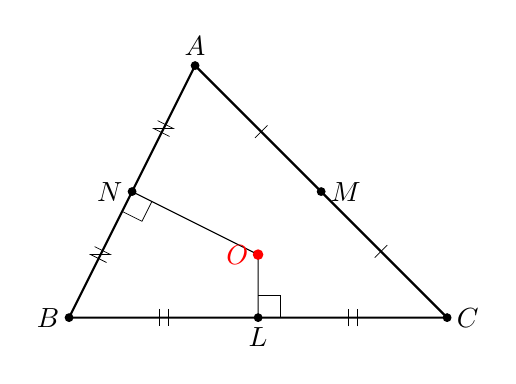
\begin{tikzpicture}[scale=1.6]
  % Define the vertices
  \coordinate (B) at (0,0);
  \coordinate (C) at (3,0);
  \coordinate (A) at (1,2);
  \coordinate (L) at ($(B)!0.5!(C)$);
  \coordinate (M) at ($(A)!0.5!(C)$);
  \coordinate (N) at ($(A)!0.5!(B)$);

  % Draw the triangle
  \draw[thick] (A)--(B)--(C)--cycle;

  % Compute centroid G = (A+B+C)/3
  \coordinate (O) at (3/2,1/2);
	\draw [line width=0.25pt] ($(L)!5pt!(C)$) -- ($(L)!5pt!(C)!5pt!90:(C)$) -- ($(L)!5pt!90:(C)$);
	%\draw [line width=0.25pt] ($(M)!5pt!(A)$) -- ($(M)!5pt!(A)!5pt!90:(A)$) -- ($(M)!5pt!90:(A)$);
	\draw [line width=0.25pt] ($(N)!5pt!(B)$) -- ($(N)!5pt!(B)!5pt!90:(B)$) -- ($(N)!5pt!90:(B)$);

	\draw [line width=0.25pt] ($(L)!0.5!(C)!1pt!(L)!2pt!90:(L)$) -- ($(L)!0.5!(C)!1pt!(L)!2pt!90:(C)$) ($(L)!0.5!(C)!1pt!(C)!2pt!90:(L)$) -- ($(L)!0.5!(C)!1pt!(C)!2pt!90:(C)$);
	\draw [line width=0.25pt] ($(L)!0.5!(B)!1pt!(L)!2pt!90:(L)$) -- ($(L)!0.5!(B)!1pt!(L)!2pt!90:(B)$) ($(L)!0.5!(B)!1pt!(B)!2pt!90:(L)$) -- ($(L)!0.5!(B)!1pt!(B)!2pt!90:(B)$);
	\draw [line width=0.25pt] ($(M)!0.5!(A)!1pt!(M)!2pt!90:(M)$) -- ($(M)!0.5!(A)!1pt!(M)!2pt!90:(A)$) ;
	\draw [line width=0.25pt] ($(M)!0.5!(C)!1pt!(M)!2pt!90:(M)$) -- ($(M)!0.5!(C)!1pt!(M)!2pt!90:(C)$) ;
	\draw [line width=0.25pt] ($(N)!0.5!(A)!1pt!(N)!2pt!90:(N)$) -- ($(N)!0.5!(A)!1pt!(N)!2pt!90:(A)$) -- ($(N)!0.5!(A)!1pt!(A)!2pt!90:(N)$) -- ($(N)!0.5!(A)!1pt!(A)!2pt!90:(A)$);
	\draw [line width=0.25pt] ($(N)!0.5!(B)!1pt!(N)!2pt!90:(N)$) -- ($(N)!0.5!(B)!1pt!(N)!2pt!90:(B)$) -- ($(N)!0.5!(B)!1pt!(B)!2pt!90:(N)$) -- ($(N)!0.5!(B)!1pt!(B)!2pt!90:(B)$);

	 %\draw (O) circle (1.58);
  % Draw medians
  \draw[] (L)--(O);
  %\draw[dashed] (M)--(O);
  \draw[] (N)--(O);
  %\draw[dashed] (A)--(O);

  % Mark the points
  \fill (A) circle (1pt) node[above] {$A$};
  \fill (B) circle (1pt) node[left] {$B$};
  \fill (C) circle (1pt) node[right] {$C$};
  \fill (L) circle (1pt) node[below] {$L$};
  \fill (M) circle (1pt) node[right] {$M$};
  \fill (N) circle (1pt) node[left] {$N$};
  \fill[red] (O) circle (1.2pt) node[left] {$O$};
\end{tikzpicture}
\end{center}
\end{frame}

\begin{frame}{証明}
$AO,BO,CO$を引くと
	\begin{center}
	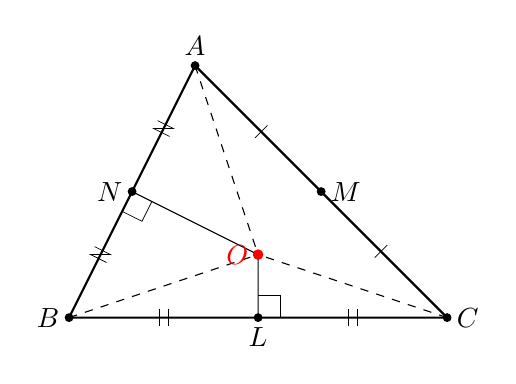
\begin{tikzpicture}[scale=1.6]
  % Define the vertices
  \coordinate (B) at (0,0);
  \coordinate (C) at (3,0);
  \coordinate (A) at (1,2);
  \coordinate (L) at ($(B)!0.5!(C)$);
  \coordinate (M) at ($(A)!0.5!(C)$);
  \coordinate (N) at ($(A)!0.5!(B)$);

  % Draw the triangle
  \draw[thick] (A)--(B)--(C)--cycle;

  % Compute centroid G = (A+B+C)/3
  \coordinate (O) at (3/2,1/2);
	\draw [line width=0.25pt] ($(L)!5pt!(C)$) -- ($(L)!5pt!(C)!5pt!90:(C)$) -- ($(L)!5pt!90:(C)$);
	%\draw [line width=0.25pt] ($(M)!5pt!(A)$) -- ($(M)!5pt!(A)!5pt!90:(A)$) -- ($(M)!5pt!90:(A)$);
	\draw [line width=0.25pt] ($(N)!5pt!(B)$) -- ($(N)!5pt!(B)!5pt!90:(B)$) -- ($(N)!5pt!90:(B)$);

	\draw [line width=0.25pt] ($(L)!0.5!(C)!1pt!(L)!2pt!90:(L)$) -- ($(L)!0.5!(C)!1pt!(L)!2pt!90:(C)$) ($(L)!0.5!(C)!1pt!(C)!2pt!90:(L)$) -- ($(L)!0.5!(C)!1pt!(C)!2pt!90:(C)$);
	\draw [line width=0.25pt] ($(L)!0.5!(B)!1pt!(L)!2pt!90:(L)$) -- ($(L)!0.5!(B)!1pt!(L)!2pt!90:(B)$) ($(L)!0.5!(B)!1pt!(B)!2pt!90:(L)$) -- ($(L)!0.5!(B)!1pt!(B)!2pt!90:(B)$);
	\draw [line width=0.25pt] ($(M)!0.5!(A)!1pt!(M)!2pt!90:(M)$) -- ($(M)!0.5!(A)!1pt!(M)!2pt!90:(A)$) ;
	\draw [line width=0.25pt] ($(M)!0.5!(C)!1pt!(M)!2pt!90:(M)$) -- ($(M)!0.5!(C)!1pt!(M)!2pt!90:(C)$) ;
	\draw [line width=0.25pt] ($(N)!0.5!(A)!1pt!(N)!2pt!90:(N)$) -- ($(N)!0.5!(A)!1pt!(N)!2pt!90:(A)$) -- ($(N)!0.5!(A)!1pt!(A)!2pt!90:(N)$) -- ($(N)!0.5!(A)!1pt!(A)!2pt!90:(A)$);
	\draw [line width=0.25pt] ($(N)!0.5!(B)!1pt!(N)!2pt!90:(N)$) -- ($(N)!0.5!(B)!1pt!(N)!2pt!90:(B)$) -- ($(N)!0.5!(B)!1pt!(B)!2pt!90:(N)$) -- ($(N)!0.5!(B)!1pt!(B)!2pt!90:(B)$);

	 %\draw (O) circle (1.58);
  % Draw medians
  \draw[] (L)--(O);
  %\draw[dashed] (M)--(O);
  \draw[] (N)--(O);
  \draw[dashed] (B)--(O);
  \draw[dashed] (C)--(O);
  \draw[dashed] (A)--(O);
  %\draw[dashed] (A)--(O);

  % Mark the points
  \fill (A) circle (1pt) node[above] {$A$};
  \fill (B) circle (1pt) node[left] {$B$};
  \fill (C) circle (1pt) node[right] {$C$};
  \fill (L) circle (1pt) node[below] {$L$};
  \fill (M) circle (1pt) node[right] {$M$};
  \fill (N) circle (1pt) node[left] {$N$};
  \fill[red] (O) circle (1.2pt) node[left] {$O$};
\end{tikzpicture}
\end{center}
準備より,$O$は垂直二等分線上にあるので$AO = BO = CO$\\
$AO = CO$から$O$が$AC$の垂直二等分線上にあることがわかる.\blacksquare
\end{frame}

\begin{frame}{外接円}
	\begin{block}{外接円}
		頂点$A,B,C$を通る円を外接円という.
	\end{block}
	証明から$AO = BO = CO$がわかったので,$O$を中心として$A,B,C$を通る円が存在する.
	\begin{center}
	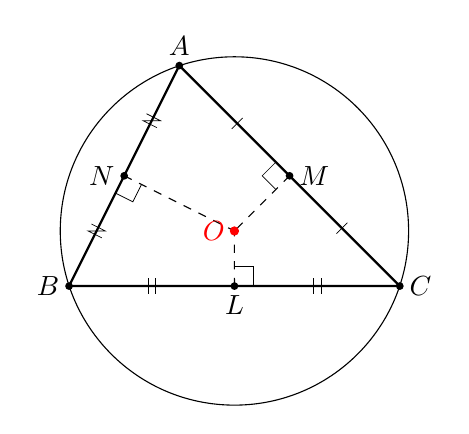
\begin{tikzpicture}[scale=1.4]
  % Define the vertices
  \coordinate (B) at (0,0);
  \coordinate (C) at (3,0);
  \coordinate (A) at (1,2);
  \coordinate (L) at ($(B)!0.5!(C)$);
  \coordinate (M) at ($(A)!0.5!(C)$);
  \coordinate (N) at ($(A)!0.5!(B)$);

  % Draw the triangle
  \draw[thick] (A)--(B)--(C)--cycle;

  % Compute centroid G = (A+B+C)/3
  \coordinate (O) at (3/2,1/2);
	\draw [line width=0.25pt] ($(L)!5pt!(C)$) -- ($(L)!5pt!(C)!5pt!90:(C)$) -- ($(L)!5pt!90:(C)$);
	\draw [line width=0.25pt] ($(M)!5pt!(A)$) -- ($(M)!5pt!(A)!5pt!90:(A)$) -- ($(M)!5pt!90:(A)$);
	\draw [line width=0.25pt] ($(N)!5pt!(B)$) -- ($(N)!5pt!(B)!5pt!90:(B)$) -- ($(N)!5pt!90:(B)$);

	\draw [line width=0.25pt] ($(L)!0.5!(C)!1pt!(L)!2pt!90:(L)$) -- ($(L)!0.5!(C)!1pt!(L)!2pt!90:(C)$) ($(L)!0.5!(C)!1pt!(C)!2pt!90:(L)$) -- ($(L)!0.5!(C)!1pt!(C)!2pt!90:(C)$);
	\draw [line width=0.25pt] ($(L)!0.5!(B)!1pt!(L)!2pt!90:(L)$) -- ($(L)!0.5!(B)!1pt!(L)!2pt!90:(B)$) ($(L)!0.5!(B)!1pt!(B)!2pt!90:(L)$) -- ($(L)!0.5!(B)!1pt!(B)!2pt!90:(B)$);
	\draw [line width=0.25pt] ($(M)!0.5!(A)!1pt!(M)!2pt!90:(M)$) -- ($(M)!0.5!(A)!1pt!(M)!2pt!90:(A)$) ;
	\draw [line width=0.25pt] ($(M)!0.5!(C)!1pt!(M)!2pt!90:(M)$) -- ($(M)!0.5!(C)!1pt!(M)!2pt!90:(C)$) ;
	\draw [line width=0.25pt] ($(N)!0.5!(A)!1pt!(N)!2pt!90:(N)$) -- ($(N)!0.5!(A)!1pt!(N)!2pt!90:(A)$) -- ($(N)!0.5!(A)!1pt!(A)!2pt!90:(N)$) -- ($(N)!0.5!(A)!1pt!(A)!2pt!90:(A)$);
	\draw [line width=0.25pt] ($(N)!0.5!(B)!1pt!(N)!2pt!90:(N)$) -- ($(N)!0.5!(B)!1pt!(N)!2pt!90:(B)$) -- ($(N)!0.5!(B)!1pt!(B)!2pt!90:(N)$) -- ($(N)!0.5!(B)!1pt!(B)!2pt!90:(B)$);

	 \draw (O) circle (1.58);
  % Draw medians
  \draw[dashed] (L)--(O);
  \draw[dashed] (M)--(O);
  \draw[dashed] (N)--(O);
  %\draw[dashed] (A)--(O);

  % Mark the points
  \fill (A) circle (1pt) node[above] {$A$};
  \fill (B) circle (1pt) node[left] {$B$};
  \fill (C) circle (1pt) node[right] {$C$};
  \fill (L) circle (1pt) node[below] {$L$};
  \fill (M) circle (1pt) node[right] {$M$};
  \fill (N) circle (1pt) node[left] {$N$};
  \fill[red] (O) circle (1.2pt) node[left] {$O$};
\end{tikzpicture}
\end{center}
	
\end{frame}
% Section 3
\section{内心}
\begin{frame}{内心の定義}
	\begin{block}{内心}
	三角形の3つの内角の二等分線が交わる点.
	\end{block}
\begin{center}
	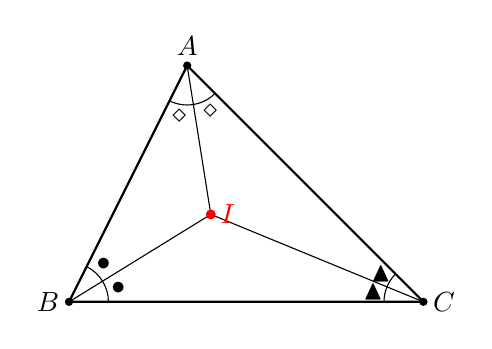
\begin{tikzpicture}[scale=1.5]
  % Define the vertices
  \coordinate (B) at (0,0);
  \coordinate (C) at (3,0);
  \coordinate (A) at (1,2);

  % Draw the triangle
  \draw[thick] (A)--(B)--(C)--cycle;

  % Compute centroid G = (A+B+C)/3
  \coordinate (I) at (1.2,0.74);
  \coordinate (L) at (1.2,0);
  \coordinate (N) at (0.54,1.08);
  \coordinate (M) at (1.73,1.27);
	 %\draw (I) circle (0.74);
  % Draw medians
  \draw[] (A)--(I);
  \draw[] (B)--(I);
	\draw[] (C)--(I);
%	\draw[dashed] (L)--(I);
%	\draw[dashed] (M)--(I);
%	\draw[dashed] (N)--(I);
  %\draw[dashed] (A)--(O);

%	\draw [line width=0.24pt] ($(L)!4pt!(C)$) -- ($(L)!4pt!(C)!4pt!90:(C)$) -- ($(L)!4pt!90:(C)$);
%	\draw [line width=0.24pt] ($(M)!4pt!(A)$) -- ($(M)!4pt!(A)!4pt!90:(A)$) -- ($(M)!4pt!90:(A)$);
%	\draw [line width=0.24pt] ($(N)!4pt!(B)$) -- ($(N)!4pt!(B)!4pt!90:(B)$) -- ($(N)!4pt!90:(B)$);

  % Mark the points
  \fill (A) circle (1pt) node[above] {$A$};
  \fill (B) circle (1pt) node[left] {$B$};
  \fill (C) circle (1pt) node[right] {$C$};
%  \fill (L) circle (1pt) node[below] {$L$};
%  \fill (M) circle (1pt) node[right] {$M$};
%  \fill (N) circle (1pt) node[left] {$N$};
  \fill[red] (I) circle (1.2pt) node[right] {$I$};

	 \path pic["$\bullet$",draw,angle radius=5mm,angle eccentricity=1.3] {angle = I--B--A};
	 \path pic["$\bullet$",draw,angle radius=5mm,angle eccentricity=1.3] {angle = C--B--I};
	 \path pic["$\diamond$",draw,angle radius=5mm,angle eccentricity=1.3] {angle = B--A--I};
	 \path pic["$\diamond$",draw,angle radius=5mm,angle eccentricity=1.3] {angle = I--A--C};
	 \path pic["$\blacktriangle$",draw,angle radius=5mm,angle eccentricity=1.3] {angle = A--C--I};
	 \path pic["$\blacktriangle$",draw,angle radius=5mm,angle eccentricity=1.3] {angle = I--C--B};
\end{tikzpicture}
\end{center}		
\end{frame}

\begin{frame}{内心}
	\begin{block}{定理4}
		三角形の3つの内角の二等分線は1点で交わる.
	\end{block}
	\begin{block}{準備}
		$P$が$\angle XOY$の二等分線上にある.\\
		$\Longleftrightarrow$ $P$と$OX$の距離と$P$と$OY$の距離が等しい.
	\end{block}
	\begin{center}
\begin{tikzpicture}[scale = 1.5]
	 \coordinate (O) at (0,0);
	 \coordinate (P) at (2.5,0);
	 \coordinate (Q) at (4,0);
  \coordinate (X) at (3,1);
  \coordinate (Y) at (3,-1);
  \coordinate (U) at (2.2,0.73);
  \coordinate (V) at (2.2,-0.73);
  \fill (X) circle (1pt) node[above] {$X$};
  \fill (Y) circle (1pt) node[below] {$Y$};
  \fill (O) circle (1pt) node[left] {$O$};
  \fill (P) circle (1pt) node[above right] {$P$};
  \draw[] (O)--(X);
  \draw[] (O)--(Y);
  \draw[] (O)--(Q);
  \draw[dashed] (P)--(U);
  \draw[dashed] (P)--(V);
	\draw [line width=0.25pt] ($(U)!5pt!(O)$) -- ($(U)!5pt!(O)!5pt!90:(O)$) -- ($(U)!5pt!90:(O)$);
	\draw [line width=0.25pt] ($(V)!5pt!(P)$) -- ($(V)!5pt!(P)!5pt!90:(P)$) -- ($(V)!5pt!90:(P)$);
	 \path pic["$\bullet$",draw,angle radius=5mm,angle eccentricity=1.3] {angle = Y--O--P};
	 \path pic["$\bullet$",draw,angle radius=5mm,angle eccentricity=1.3] {angle = P--O--X};
\end{tikzpicture}
	\end{center}
\end{frame}

\begin{frame}{証明}
	$I$から,各辺に垂線をおろす.
\begin{center}
	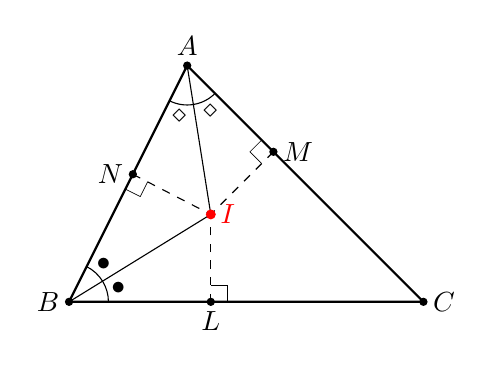
\begin{tikzpicture}[scale=1.5]
  % Define the vertices
  \coordinate (B) at (0,0);
  \coordinate (C) at (3,0);
  \coordinate (A) at (1,2);

  % Draw the triangle
  \draw[thick] (A)--(B)--(C)--cycle;

  % Compute centroid G = (A+B+C)/3
  \coordinate (I) at (1.2,0.74);
  \coordinate (L) at (1.2,0);
  \coordinate (N) at (0.54,1.08);
  \coordinate (M) at (1.73,1.27);
	 %\draw (I) circle (0.74);
  % Draw medians
  \draw[] (A)--(I);
  \draw[] (B)--(I);
	%\draw[] (C)--(I);
	\draw[dashed] (L)--(I);
	\draw[dashed] (M)--(I);
	\draw[dashed] (N)--(I);
  %\draw[dashed] (A)--(O);

	\draw [line width=0.24pt] ($(L)!4pt!(C)$) -- ($(L)!4pt!(C)!4pt!90:(C)$) -- ($(L)!4pt!90:(C)$);
	\draw [line width=0.24pt] ($(M)!4pt!(A)$) -- ($(M)!4pt!(A)!4pt!90:(A)$) -- ($(M)!4pt!90:(A)$);
	\draw [line width=0.24pt] ($(N)!4pt!(B)$) -- ($(N)!4pt!(B)!4pt!90:(B)$) -- ($(N)!4pt!90:(B)$);

  % Mark the points
  \fill (A) circle (1pt) node[above] {$A$};
  \fill (B) circle (1pt) node[left] {$B$};
  \fill (C) circle (1pt) node[right] {$C$};
  \fill (L) circle (1pt) node[below] {$L$};
  \fill (M) circle (1pt) node[right] {$M$};
  \fill (N) circle (1pt) node[left] {$N$};
  \fill[red] (I) circle (1.2pt) node[right] {$I$};

	 \path pic["$\bullet$",draw,angle radius=5mm,angle eccentricity=1.3] {angle = I--B--A};
	 \path pic["$\bullet$",draw,angle radius=5mm,angle eccentricity=1.3] {angle = C--B--I};
	 \path pic["$\diamond$",draw,angle radius=5mm,angle eccentricity=1.3] {angle = B--A--I};
	 \path pic["$\diamond$",draw,angle radius=5mm,angle eccentricity=1.3] {angle = I--A--C};
%	 \path pic["$\blacktriangle$",draw,angle radius=5mm,angle eccentricity=1.3] {angle = A--C--I};
%	 \path pic["$\blacktriangle$",draw,angle radius=5mm,angle eccentricity=1.3] {angle = I--C--B};
\end{tikzpicture}
\end{center}
準備の$(\Longrightarrow)$より,$IN = IL = IM$.	
\end{frame}

\begin{frame}{証明}
	$I$から$C$に線分を引く.
	\begin{center}
	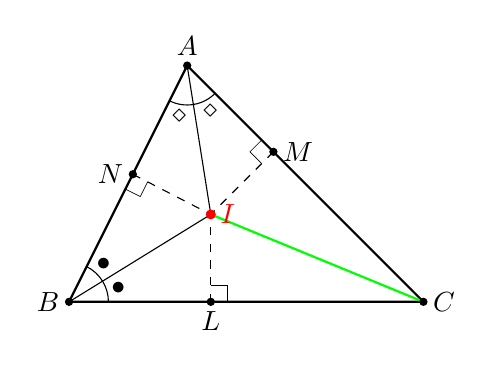
\begin{tikzpicture}[scale=1.5]
  % Define the vertices
  \coordinate (B) at (0,0);
  \coordinate (C) at (3,0);
  \coordinate (A) at (1,2);

  % Draw the triangle
  \draw[thick] (A)--(B)--(C)--cycle;

  % Compute centroid G = (A+B+C)/3
  \coordinate (I) at (1.2,0.74);
  \coordinate (L) at (1.2,0);
  \coordinate (N) at (0.54,1.08);
  \coordinate (M) at (1.73,1.27);
	 %\draw (I) circle (0.74);
  % Draw medians
  \draw[] (A)--(I);
  \draw[] (B)--(I);
	\draw[thick, green] (C)--(I);
	\draw[dashed] (L)--(I);
	\draw[dashed] (M)--(I);
	\draw[dashed] (N)--(I);
  %\draw[dashed] (A)--(O);

	\draw [line width=0.24pt] ($(L)!4pt!(C)$) -- ($(L)!4pt!(C)!4pt!90:(C)$) -- ($(L)!4pt!90:(C)$);
	\draw [line width=0.24pt] ($(M)!4pt!(A)$) -- ($(M)!4pt!(A)!4pt!90:(A)$) -- ($(M)!4pt!90:(A)$);
	\draw [line width=0.24pt] ($(N)!4pt!(B)$) -- ($(N)!4pt!(B)!4pt!90:(B)$) -- ($(N)!4pt!90:(B)$);

  % Mark the points
  \fill (A) circle (1pt) node[above] {$A$};
  \fill (B) circle (1pt) node[left] {$B$};
  \fill (C) circle (1pt) node[right] {$C$};
  \fill (L) circle (1pt) node[below] {$L$};
  \fill (M) circle (1pt) node[right] {$M$};
  \fill (N) circle (1pt) node[left] {$N$};
  \fill[red] (I) circle (1.2pt) node[right] {$I$};

	 \path pic["$\bullet$",draw,angle radius=5mm,angle eccentricity=1.3] {angle = I--B--A};
	 \path pic["$\bullet$",draw,angle radius=5mm,angle eccentricity=1.3] {angle = C--B--I};
	 \path pic["$\diamond$",draw,angle radius=5mm,angle eccentricity=1.3] {angle = B--A--I};
	 \path pic["$\diamond$",draw,angle radius=5mm,angle eccentricity=1.3] {angle = I--A--C};
%	 \path pic["$\blacktriangle$",draw,angle radius=5mm,angle eccentricity=1.3] {angle = A--C--I};
%	 \path pic["$\blacktriangle$",draw,angle radius=5mm,angle eccentricity=1.3] {angle = I--C--B};
\end{tikzpicture}
\end{center}
$IM = IL$なので,準備の$(\Longleftarrow)$より,$IC$は$\angle MCL$の二等分線になっている.\blacksquare
\end{frame}

\begin{frame}{内接円}
	\begin{block}{内接円の定義を求めよ.}
	$IM = IN = IL$で各辺と垂直に交わるので,$I$を中心として3辺に接する円が存在し,これを\textbf{内接円}と呼ぶ.
	\end{block}
\begin{center}
	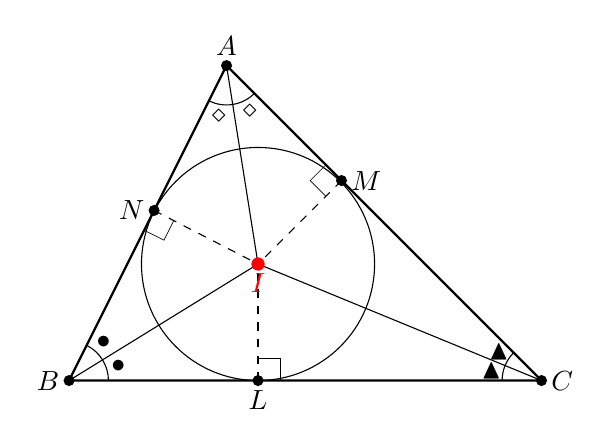
\begin{tikzpicture}[scale=2]
  % Define the vertices
  \coordinate (B) at (0,0);
  \coordinate (C) at (3,0);
  \coordinate (A) at (1,2);

  % Draw the triangle
  \draw[thick] (A)--(B)--(C)--cycle;

  % Compute centroid G = (A+B+C)/3
  \coordinate (I) at (1.2,0.74);
  \coordinate (L) at (1.2,0);
  \coordinate (N) at (0.54,1.08);
  \coordinate (M) at (1.73,1.27);
	 \draw (I) circle (0.74);
  % Draw medians
  \draw[] (A)--(I);
  \draw[] (B)--(I);
	\draw[] (C)--(I);
	\draw[dashed] (L)--(I);
	\draw[dashed] (M)--(I);
	\draw[dashed] (N)--(I);
  %\draw[dashed] (A)--(O);

	\draw [line width=0.24pt] ($(L)!4pt!(C)$) -- ($(L)!4pt!(C)!4pt!90:(C)$) -- ($(L)!4pt!90:(C)$);
	\draw [line width=0.24pt] ($(M)!4pt!(A)$) -- ($(M)!4pt!(A)!4pt!90:(A)$) -- ($(M)!4pt!90:(A)$);
	\draw [line width=0.24pt] ($(N)!4pt!(B)$) -- ($(N)!4pt!(B)!4pt!90:(B)$) -- ($(N)!4pt!90:(B)$);

  % Mark the points
  \fill (A) circle (1pt) node[above] {$A$};
  \fill (B) circle (1pt) node[left] {$B$};
  \fill (C) circle (1pt) node[right] {$C$};
  \fill (L) circle (1pt) node[below] {$L$};
  \fill (M) circle (1pt) node[right] {$M$};
  \fill (N) circle (1pt) node[left] {$N$};
  \fill[red] (I) circle (1.2pt) node[below] {$I$};

	 \path pic["$\bullet$",draw,angle radius=5mm,angle eccentricity=1.3] {angle = I--B--A};
	 \path pic["$\bullet$",draw,angle radius=5mm,angle eccentricity=1.3] {angle = C--B--I};
	 \path pic["$\diamond$",draw,angle radius=5mm,angle eccentricity=1.3] {angle = B--A--I};
	 \path pic["$\diamond$",draw,angle radius=5mm,angle eccentricity=1.3] {angle = I--A--C};
	 \path pic["$\blacktriangle$",draw,angle radius=5mm,angle eccentricity=1.3] {angle = A--C--I};
	 \path pic["$\blacktriangle$",draw,angle radius=5mm,angle eccentricity=1.3] {angle = I--C--B};
\end{tikzpicture}
\end{center}	
	
\end{frame}

\section{垂心}
\begin{frame}{垂心}
	\begin{block}{垂心の定義}
		三角形の各頂点から対辺,もしくはその延長に下ろした垂線の交点$H$.
	\end{block}
	
	\begin{center}
		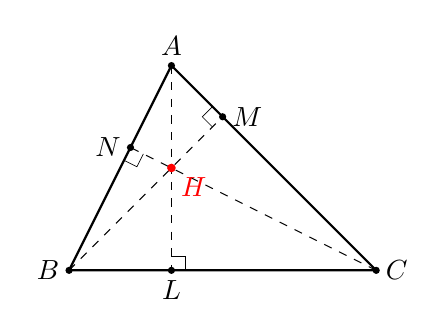
\begin{tikzpicture}[scale=1.3]
  % Define the vertices
  \coordinate (B) at (0,0);
  \coordinate (C) at (3,0);
  \coordinate (A) at (1,2);
  \coordinate (L) at (1,0);
  \coordinate (M) at (1.5,1.5);
  \coordinate (N) at (0.6,1.2);

  % Draw the triangle
  \draw[thick] (A)--(B)--(C)--cycle;

  % Compute centroid G = (A+B+C)/3
  \coordinate (H) at (1,1);

  % Draw medians
  \draw[dashed] (A)--(L);
  \draw[dashed] (B)--(M);
  \draw[dashed] (C)--(N);

  % Mark the points
  \fill (A) circle (1pt) node[above] {$A$};
  \fill (B) circle (1pt) node[left] {$B$};
  \fill (C) circle (1pt) node[right] {$C$};
  \fill (L) circle (1pt) node[below] {$L$};
  \fill (M) circle (1pt) node[right] {$M$};
  \fill (N) circle (1pt) node[left] {$N$};
  \fill[red] (H) circle (1.2pt) node[below right] {$H$};

	\draw [line width=0.24pt] ($(L)!4pt!(C)$) -- ($(L)!4pt!(C)!4pt!90:(C)$) -- ($(L)!4pt!90:(C)$);
	\draw [line width=0.24pt] ($(M)!4pt!(A)$) -- ($(M)!4pt!(A)!4pt!90:(A)$) -- ($(M)!4pt!90:(A)$);
	\draw [line width=0.24pt] ($(N)!4pt!(B)$) -- ($(N)!4pt!(B)!4pt!90:(B)$) -- ($(N)!4pt!90:(B)$);
\end{tikzpicture}
	\end{center}
\end{frame}

\section{傍心}
\begin{frame}{傍心}
	\begin{block}{傍心の定義}
		\triangle ABCの1つの内角の二等分線と,他の2つの外角の二等分線の交点.
	\end{block}
	\begin{center}
		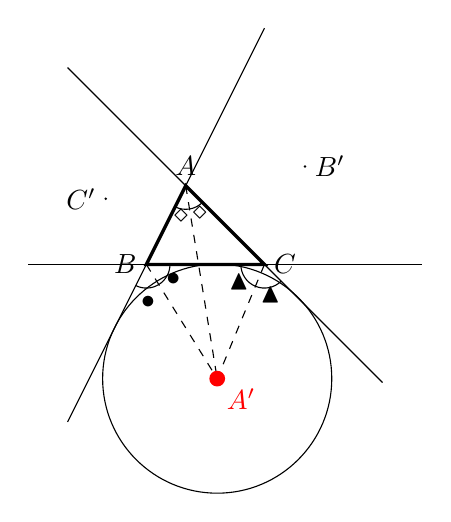
\begin{tikzpicture}[scale=0.5]
  % Define the vertices
  \coordinate (B) at (0,0);
  \coordinate (C) at (3,0);
  \coordinate (A) at (1,2);
  \coordinate (L) at (1.80,-2.90);
	\coordinate (M) at (4.03,2.49);
  \coordinate (N) at (-1.03,1.67);

  % Draw the triangle
  \draw[very thick] (A) -- (B) -- (C) -- cycle;
  \draw[] (3,6)--(-2,-4);
  \draw[] (-3,0)--(7,0);
  \draw[] (-2,5)--(6,-3);
  \coordinate (P) at (-2,-4);
	\coordinate (Q) at (6,-3);

  % Draw medians
  \draw[dashed] (A)--(L);
  \draw[dashed] (B)--(L);
  \draw[dashed] (C)--(L);


	\draw (L) circle (2.91);
	%\draw (M) circle (2.49);
	%\draw (N) circle (1.67);
  % Mark the points
  \fill (A) circle (1pt) node[above] {$A$};
  \fill (B) circle (1pt) node[left] {$B$};
  \fill (C) circle (1pt) node[right] {$C$};
  \fill[red] (L) circle (2mm) node[below right] {$A'$};
  \fill (M) circle (1pt) node[right] {$B'$};
  \fill (N) circle (1pt) node[left] {$C'$};

	 \path pic["$\bullet$",draw,angle radius=3mm,angle eccentricity=1.6] {angle = P--B--L};
	 \path pic["$\bullet$",draw,angle radius=3mm,angle eccentricity=1.3] {angle = L--B--C};
	 \path pic["$\diamond$",draw,angle radius=3mm,angle eccentricity=1.3] {angle = B--A--L};
	 \path pic["$\diamond$",draw,angle radius=3mm,angle eccentricity=1.3] {angle = L--A--C};
	 \path pic["$\blacktriangle$",draw,angle radius=3mm,angle eccentricity=1.3] {angle = L--C--Q};
	 \path pic["$\blacktriangle$",draw,angle radius=3mm,angle eccentricity=1.3] {angle = B--C--L};
\end{tikzpicture}
	\end{center}
\end{frame}

\begin{frame}{問題}
	\begin{block}{問題}
	重心と内心が一致する三角形は,正三角形であることを証明せよ.
	\end{block}
\end{frame}

\begin{frame}{Example}
  \begin{exampleblock}{Derived Category Example}
    The functor \( \mathrm{Ext}^i(-,-) \) gives a cohomological \(\delta\)-functor.
  \end{exampleblock}
\end{frame}

% Conclusion
\begin{frame}{Summary}
  \begin{enumerate}
    \item Main result
    \item Key ideas
    \item Future directions
  \end{enumerate}
\end{frame}

\begin{frame}{Summary}
  \begin{enumerate}
    \item Main result
    \item Key ideas
    \item Future directions
  \end{enumerate}
\end{frame}
\begin{frame}{Questions}
  \centering
  \Huge Questions?
\end{frame}

\end{document}
